\documentclass[11pt,a4paper]{article}
\usepackage[utf8x]{inputenc}
\usepackage{ucs}
\usepackage[francais]{babel}
\usepackage[T1]{fontenc}
\usepackage{amsmath}
\usepackage{amsfonts}
\usepackage{amssymb}
\usepackage{fullpage}
\usepackage{float}
\usepackage{listings}
\usepackage{graphicx}

\title{Rapport projet compilation : ANTLR}
\author{Mathias Millet, Gaspard Douady}
\date{M1 - 28 septembre 2011}

\begin{document}

\maketitle
\newpage

\part*{Introduction}
Dans ce projet nous avons appris les bases d'ANTLR, testé un exemple de grammaire d'évaluateur d'expression, et étendu cet evaluateur pour accepter les divisions et les puissances.

\part{Ajout des opérateurs}
Dans une première version, nous avons utilisé la même méthode pour ajouter la division que celle utilisé dans l'exemple pour gérer l'addition et la soustraction.\\
Nous avons aussi rajouté un étage entre multExpr et atom pour gérer l'opérateur de puissance.

	\section{Code}\begin{scriptsize}
	\lstinputlisting{code/Expr2.g}\end{scriptsize}
	
	\section{Grammaire utilisée}
		Nous avons donc modifié ajouté une dérivation possible à multEXPR, et ajouté la règle powEXPR :  
		\begin{center}
		 \begin{tabular}{lrl}
			multEXPR & $\longrightarrow$ & powEXPR\\
 					& ( &   * multEXPR\\
 					& | & / multEXPR $)^*$\\
			powEXPR & $\longrightarrow$ & atom  \\
					& | & atom \^{} atom
	\end{tabular}\end{center}
	Où ANTLR interprète l'opérateur $^*$ comme la génération d'une infinité de règles. Ainsi, l'expression $1-1-1$ est capturée par la règle multEXPR - multEXPR - multEXPR, qui va lui attribuer la bonne valeur.
	\section{Résultats}

Avec le debugger, tout se passe bien :\\
\begin{figure}[h!]\caption{Evalutation de l'expression 2*(((6/2)\^{}2-5) avec le debugger}
\centering
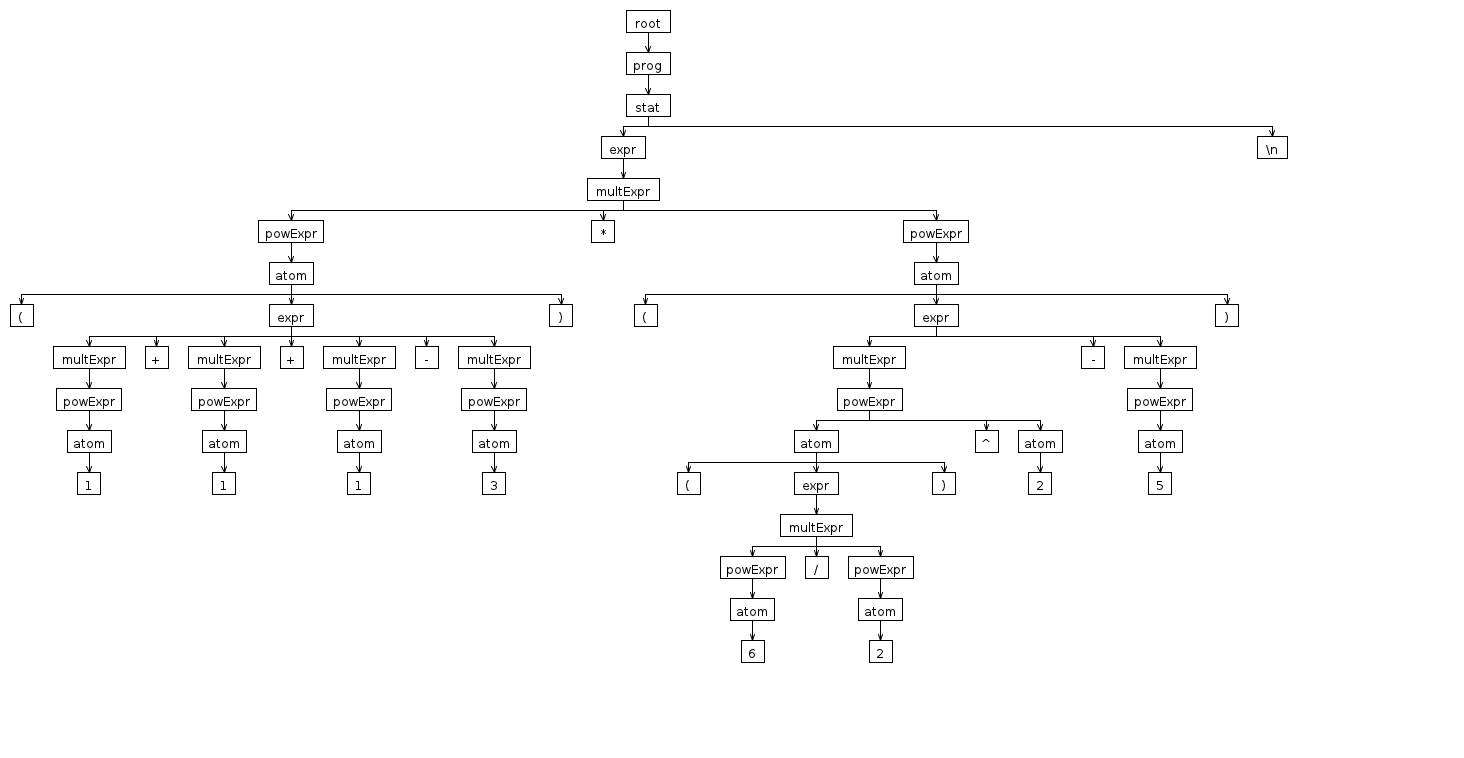
\includegraphics[scale=0.3]{figures/arbre_v1_debugger.jpg}
\end{figure}

Cette grammaire ne fonctionne cependant pas avec l'interpréteur d'ANTLRWorks, a priori car il n'intègre pas l'évalution des prédicats syntaxiques (difficulté avec * et | ).
\begin{figure}[h!]\caption{Evalutation de l'expression $1-1$ avec l'interpréteur}
\centering
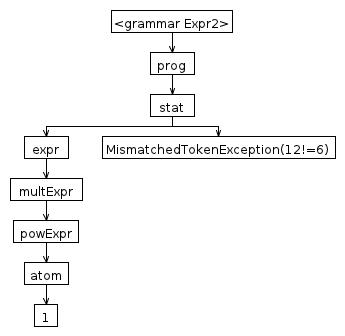
\includegraphics[scale=0.5]{figures/arbre_v1_interpreter.jpg}
\end{figure}
Nous avons donc cherché une autre grammaire qui fonctionne aussi bien avec l'interpréteur que le debugger.

\part{Modification de la grammaire}
Dans cette seconde version, nous avons choisi de modifier le problème afin de fonctionner avec des flottant et non des entiers. Le but de ce changement est de rendre la multiplication et la division inverse l'un de l'autre.\\
\subsection{Grammaire utilisée}
 \begin{tabular}{lrl}
			EXPR & $\rightarrow$ & multEXPR \\ 
 					& | & multEXPR + EXPR \\
 					& | & multEXPR - EXPR \\
\end{tabular} 
De même pour la règle multEXPR; la règle powEXPR est inchangée.
		\subsection{code}\begin{scriptsize}
		\lstinputlisting{code/Expr.g}\end{scriptsize}
		
		\subsection{Fonctionnement}		
			Le problème avec cette grammaire, récursive à droite, est que le parenthésage implicite se fait dans le mauvais sens : l'expression $1-1-1$ est interprétée comme $1-(1-1)$ et vaut donc $1$. L'idée est alors d'exploiter le fait que les opérateurs + et -sont des inverses l'un de l'autre : on va alors modifier le sens des opérateurs suivant ceux qui les précèdent : un - va transformer tous les + (resp. -) en - (resp +). $1-(1-1)$ s'évalue donc comme $1-(1+1)$ et rend le bon résultat.\\
Il fallait passer aux flottants car, dans l'algèbre des entiers, * et / ne sont pas inverses l'un de l'autre. En passant aux  flottants, tout se passe alors de la même façon.\\

		\subsection{Résultats}
Cette grammaire fonctionne donc de manière "artificielle", en changeant un peu le problème. Les résultats sont cependant bons. \\
\begin{figure}[h!]
\begin{minipage}[b]{0.5\linewidth}\centering
\caption{Evalutation de l'expression $1-1$ avec l'interpréteur}
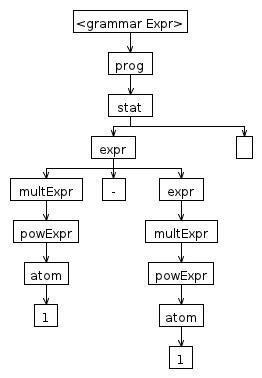
\includegraphics[scale=0.5]{figures/arbre_v2_interpreter.jpg}
\end{minipage}
\hspace{0.5cm}
\begin{minipage}{0.5\linewidth}\centering
\caption{Evalutation de l'expression $1-1$ avec le debugger}
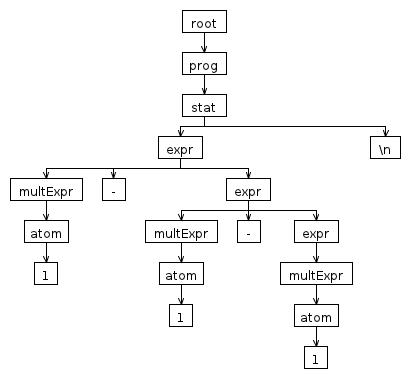
\includegraphics[scale=0.5]{figures/arbre_v2_debugger.jpg}
\end{minipage}
\end{figure}

\part{Conclusion}
La premiere version donne une grammaire correcte sur le papier mais que l'interpreteur d'AntlrWorks ne comprend pas.\\
La seconde version ne réponds pas exactement à la question posée, mais fonctionne correctement dans toutes les situations, sans avoir besoin de générer une infinité de règles.\\
Une autre solution aurait été de stocker toutes les valeurs renvoyées par les membres suivants une expression, et de calculer le résultats à la fin (comme vu en TD).
\end{document}